\section{How does sampling work?}
\label{sec:hws_how}

While the last section was concerned with \textit{what} the hws library can sample, this section explains \textit{how} it is implemented. 
If one is only interested in how to use the hws library, the next \autoref{sec:hws_example} will showcase an example usage of the hws library. 

The general internal flow of the hws library looks as follows. 
When the first hardware sampler for a specific hardware platform is constructed, the required environment from the respective vendor library is initialized. 
Using an atomic reference count also ensures that the environments are only initialized once, even when multiple hardware samplers for the same hardware type are used. 

The general flow of the hws library looks as follows:
\begin{enumerate}
    % \item%
    % A new hardware sampler is constructed, initializing the required environment from the respective vendor library. 
    % An atomic reference count is used to ensure that the respective environments are only initialized once. 
    % Note that it is supported to start as many hardware samplers as one wishes and that combination of different hardware samplers is supported. 
    % If everything should be sampled, it is easiest to use a \code{system_hardware_sampler}.
    \item%
    A hardware sampler is then started using the \code{start_sampling()} function which internally spawns a new \code{std::thread}. 
    The actual sampling process then takes place asynchronously in this newly created thread. 
    Note that one thread is created for each hardware sampler. 
    The \code{system_hardware_sampler} also starts as many threads as it encapsulates other hardware samplers. 
    \item%
    All supported hardware samples are initialized: The fixed samples to their final values and the running samples to their first value. 
    This step is also used to determine which hardware samples are supported on the current hardware. 
    All theoretically by hws supported samples are queried and if the respective vendor function returns with an error, i.e., a sample is not supported, the value will be set to an \code{std::nullopt} indicating that it can be ignored in future sampling attempts during the sampling loop. 
    \item%
    The actual sampling loop is started. 
    Here, a new value is added to every supported running sample. 
    At the end, the current thread sleeps for the amount of time specified by the sampling interval before it starts again to sample new values. 
    Using the \code{pause_sampling()} and \code{resume_sampling()} functions, the sampling of new values can temporarily be paused using an atomic flag as a signaling variable. 
    \item%
    At the end, one must call the \code{stop_sampling()} function which waits until the current sampling loop has finished and then joins on the previously spawned \code{std::thread}. 
    Note that once a hardware sampler has been stopped, it cannot be started again. 
    \item%
    Only after the hardware sampler has been stopped, all samples can be saved to a YAML file using the \code{dump_yaml(filename)} function. 
    Note that it is still possible to retrieve the current hardware samples programmatically during the program execution.
    \item%
    At the end of the lifetime of a hardware sampler, in its constructor the previously mentioned reference count is decreased and only if it reaches zero, the respective vendor specific environment is shut down ensuring this only happens once. 
\end{enumerate}

\todo{remake plot (new runtimes with more data points)}
\begin{figure}
    \centering
    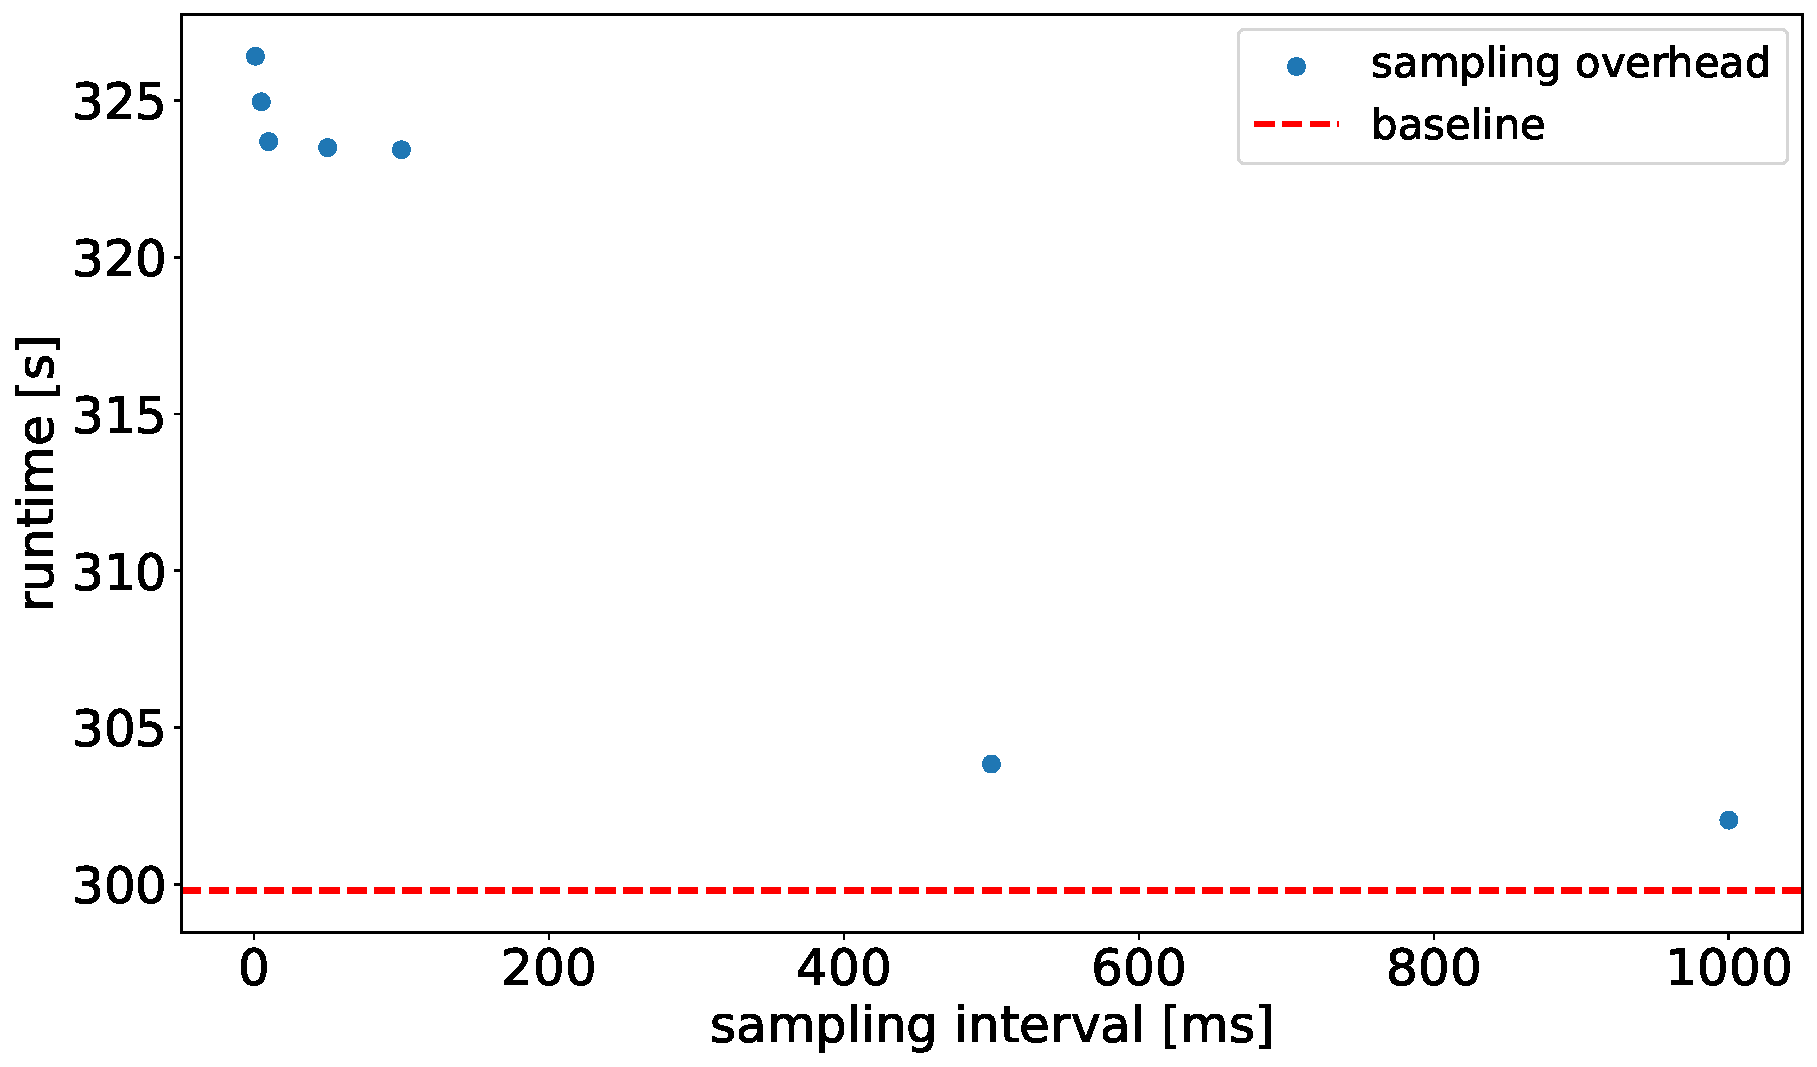
\includegraphics[width=0.8\linewidth]{figures/03_performance_sampling_hws/hws_sampling_interval_overhead.pdf}
    \caption{%
    The overhead when using the hws library, depends on the specified sampling interval. 
    The red dashed line at the bottom is the baseline version without hws. 
    We can see, that the overhead when using hws is noticeable for smaller sampling intervals. 
    However, increasing the sampling interval also drastically decreases the overhead. 
    }
    \label{fig:hws_overhead}
\end{figure}


\subsection{Implementation on GPUs}
\label{sec:hws_impl_gpus}

For implementing hws on the supported \glspl{gpu}, vendor-specific libraries are used. 
To sample information on NVIDIA \glspl{gpu} \gls{nvml}~\cite{nvidia_nvml_2024} is used, on \gls{amd} \glspl{gpu} the \gls{rocmsmi} library~\cite{amd_rocm_2024}, and on Intel \glspl{gpu} the Level Zero library~\cite{intel_level_2024}. 
While the \gls{nvml} and \gls{rocmsmi} \glspl{api} are relatively similar, Level Zero has a significantly different approach that can also be seen in \autoref{code:vendor_library_calls}. 
All library functions return a status code indicating whether the \gls{api} call was successful. 
If requested during CMake configuration, hws internally checks these status codes and raises an error if a function fails.  
Additionally, the \gls{nvml} and Level Zero specific device handles are wrapped in a custom wrapper class to prevent implementation details from leaking into the public headers. 

\subsection{Implementation on CPUs}
\label{sec:hws_impl_cpus}

On the \gls{cpu}, however, this is different since there is no simple library that can be called to gather all the necessary information. 
Therefore, three different command-line utilities are used if and only if they can be found during CMake configuration; otherwise, all related code is ignored, and the respective samples are not gathered. 
To retrieve general \gls{cpu} information, like the core count, socket count, or cache size, \texttt{lscpu}~\cite{qian_lscpu_nodate} is used, for memory-related information, i.e., available, used, and total main memory, the \texttt{free}~\cite{small_free_nodate} utility is used, and for everything else, like frequency or power related information, \texttt{turbostat}~\cite{brown_turbostat_nodate} is used. 
In all three cases, the \textit{subprocess.h} library~\cite{henning_subprocessh_2024} is used to create a new subprocess that, in turn, executes the respective utility, returning the standard output as a string, which is then post-processed, extracting the necessary information inside the \gls{cpu} hardware sampler.  

% lscpu
In case of the \texttt{lscpu} utility, the subprocess simply calls \texttt{lscpu}. 
Note that the cache sizes are only reported as strings instead of integers containing the actual values since the \texttt{lscpu} output is not standardized and varies greatly between \glspl{cpu}. 
%
% free
For the \texttt{free} utility, the command-line flag \texttt{-b} is added to ensure that the memory sizes are output in bytes. 

%turbostat
For \texttt{turbostat}, it is a bit more difficult. 
First, it should be noted that to get the full \texttt{turbostat} information, it has to be executed with root privileges. 
However, in newer \texttt{turbostat} versions, it is possible to get a subset of all possible information even if \texttt{turbostat} is not called with root privileges. 
The hws library handles this distinction during CMake configuration. 
If \texttt{turbostat} can be used with root privileges, the command \code{sudo turbostat -n 1 -i 0.001 -S -q} is executed; if root privileges are not granted, \code{sudo} is omitted. 
This command samples all available information immediately (\code{-i 0.001}) exactly once (\code{-n 1}) and outputs the information in a short summary format (\code{-S}), skipping potential header information (\code{-q}). 
An example \texttt{turbostat} output with the mentioned command is displayed in \autoref{code:turbostat_output}. 
\begin{listing}
    \begin{moderncode}{text}
Avg_MHz  Busy%  Bzy_MHz  TSC_MHz  IPC   IRQ  POLL  C1   C2   POLL%  C1%   C2%     CorWatt  PkgWatt
39       1.77   2212     4686     0.92  818  1     156  819  0.01   3.03  110.73  4.58     264.06
    \end{moderncode}
    \caption{%
    An example output of the turbostat command \code{sudo turbostat -n 1 -i 0.001 -S -q} with root privileges enabled on an \gls{amd} EPYC 9274F \gls{cpu}.
    }
    \label{code:turbostat_output}
\end{listing}
Note that the output of \texttt{turbostat} also depends on the used \gls{cpu}. 
For example, the output in \autoref{code:turbostat_output} was gathered on an \gls{amd} EPYC 9274F \gls{cpu} and consists of $14$ table entries. 
The same command executed on an Intel i5-10210U \gls{cpu}, the output consists of $52$ columns, mostly adding more idle state information but also temperature-related information missing for the \gls{amd} \gls{cpu}.

